%% LaTeX-Beamer template for KIT design
%% by Erik Burger, Christian Hammer
%% title picture by Klaus Krogmann
%%
%% version 2.1
%%
%% mostly compatible to KIT corporate design v2.0
%% http://intranet.kit.edu/gestaltungsrichtlinien.php
%%
%% Problems, bugs and comments to
%% burger@kit.edu

\documentclass[18pt]{beamer}

%% SLIDE FORMAT

% use 'beamerthemekit' for standard 4:3 ratio
% for widescreen slides (16:9), use 'beamerthemekitwide'

% \usepackage{templates/beamerthemekitwide}

%% TITLE PICTURE

% if a custom picture is to be used on the title page, copy it into the 'logos'
% directory, in the line below, replace 'mypicture' with the
% filename (without extension) and uncomment the following line
% (picture proportions: 63 : 20 for standard, 169 : 40 for wide
% *.eps format if you use latex+dvips+ps2pdf,
% *.jpg/*.png/*.pdf if you use pdflatex)

%\titleimage{adversarial_overview}


%% TITLE LOGO

% for a custom logo on the front page, copy your file into the 'logos'
% directory, insert the filename in the line below and uncomment it

%\titlelogo{mylogo}

% (*.eps format if you use latex+dvips+ps2pdf,
% *.jpg/*.png/*.pdf if you use pdflatex)

%% TikZ INTEGRATION

% use these packages for PCM symbols and UML classes
% \usepackage{templates/tikzkit}
% \usepackage{templates/tikzuml}

% the presentation starts here

\title[A brief outlook]{A brief outlook}
%\subtitle{Applied and Algorithmic Views on Machine Learning, Figure below from \cite{goodfellow14}}
\author{Leander Kurscheidt}

%\institute{INSTITUTE FOR PROGRAM STRUCTURES AND DATA ORGANIZATION · CHAIR FOR SYSTEMS OF INFORMATIONMANAGEMENT}

\usepackage{amsmath}
\usepackage{pgfplots}
\usepgfplotslibrary{fillbetween}
\usepackage{mathtools,amssymb}
\usepackage{tikz}
%adapted from https://tex.stackexchange.com/questions/352933/drawing-a-normal-distribution-graph
\pgfmathdeclarefunction{gauss}{2}{\pgfmathparse{1/(#2*sqrt(2*pi))*exp(-((x-#1)^2)/(2*#2^2))}%
}
\pgfmathdeclarefunction{gaussError}{0}{%
  \pgfmathparse{%
    (x<=(-2))*(gauss(-2.5,1)-0.3) +%
    (x>(-2))*gauss(0, 1)}}

\usepackage{xcolor}

\graphicspath{ {images/} }

% Bibliography

%\usepackage[citestyle=authoryear,bibstyle=numeric,hyperref,backend=biber]{biblatex}
\usepackage[citestyle=alphabetic,bibstyle=numeric,hyperref,backend=biber]{biblatex}
\addbibresource{templates/example.bib}
\bibhang1em

\begin{document}

% change the following line to "ngerman" for German style date and logos
\selectlanguage{english}

%title page
\begin{frame}
\titlepage
\end{frame}

%table of contents
%\begin{frame}{Outline/Gliederung}
%\tableofcontents
%\end{frame}

\section{Batches}
\begin{frame}
    \vfill
    \centering
    \begin{beamercolorbox}[sep=8pt,center,shadow=true,rounded=true]{title}
      \usebeamerfont{title}We normally learn in batches
    \end{beamercolorbox}
    \vfill
\end{frame}

\section{GAN}
\begin{frame}
    \vfill
    \centering
    \begin{beamercolorbox}[sep=8pt,center,shadow=true,rounded=true]{title}
      \usebeamerfont{title}GANs
    \end{beamercolorbox}
    \vfill
\end{frame}

\begin{frame}{Introduction to generative models}
\begin{figure}[h]
    \centering
    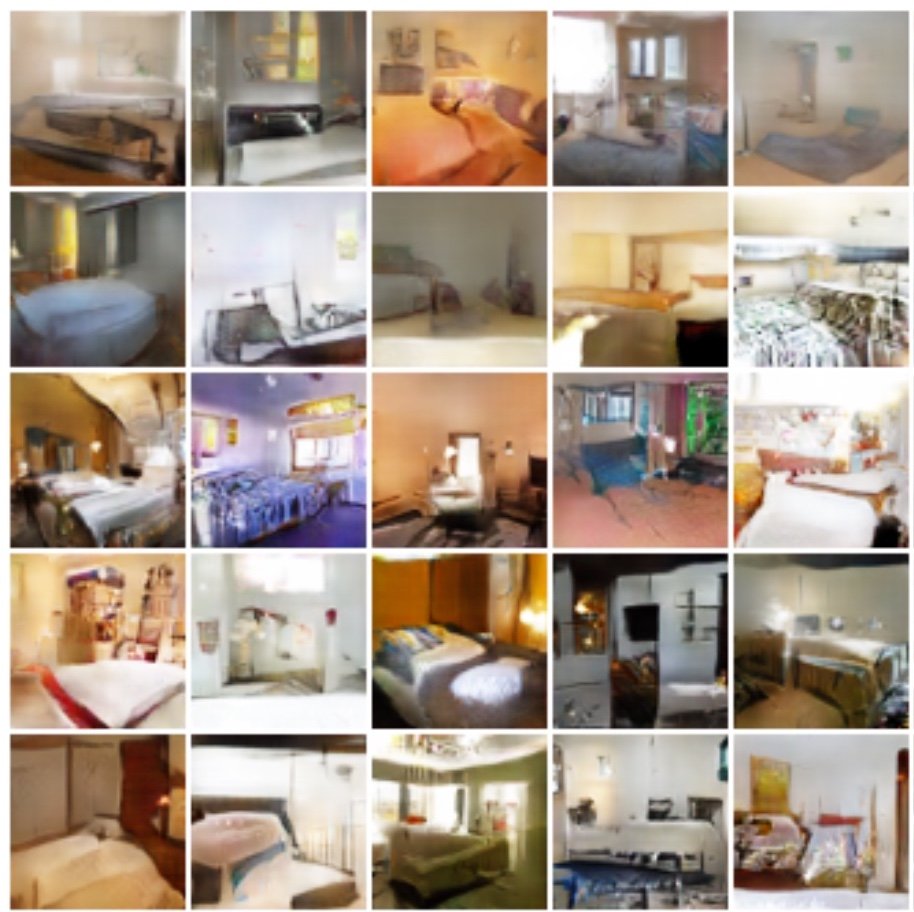
\includegraphics[width=1\textwidth,height=0.6\textheight,keepaspectratio]{wasserstein_examples_crop}
    \caption{Samples from a Wasserstein-GAN, Selection from a figure from \cite{ArjovskyCB17}}
\end{figure}
\end{frame}

\begin{frame}{Introduction to generative models}
In our context an (optimal) generative model is a function
\begin{align*}
    G : P_{z} \to P_{data}
\end{align*}
where $P_{z}$ is an arbitrary distribution, often called noise-distribution. %, like $\mathcal{N}(\mu,\,\sigma^{2})$.
$P_{data}$ is the distribution we want to sample from.
\end{frame}

\begin{frame}{Generative Adversarial Networks}
as formulated by \cite{goodfellow14}:\\
\vfill
\begin{minipage}[t]{0.48\linewidth}
    \textbf{discriminative model $D(x; \theta_d)$}\\
    tries to:
    \begin{itemize}
        \item assign 1 to elements of the original data
        \item assign 0 to elements produced by the generator
        \item \textit{``tries distinguish real and generated samples"}
    \end{itemize}
\end{minipage}
\hfill
\begin{minipage}[t]{0.48\linewidth}
    \textbf{generative model $G(z; \theta_g)$}\\
    tries to:
    \begin{itemize}
        \item maximize $D(G(z))$
        \item \textit{``tries to generate samples that fool the discriminator"}
    \end{itemize}
\end{minipage}
\vfill
GANs converge to a Nash-Equilibrium, as shown by \cite{HeuselRUNKH17}.
\end{frame}

\begin{frame}{Generative Adversarial Networks}
    \begin{figure}[h]
    \centering
    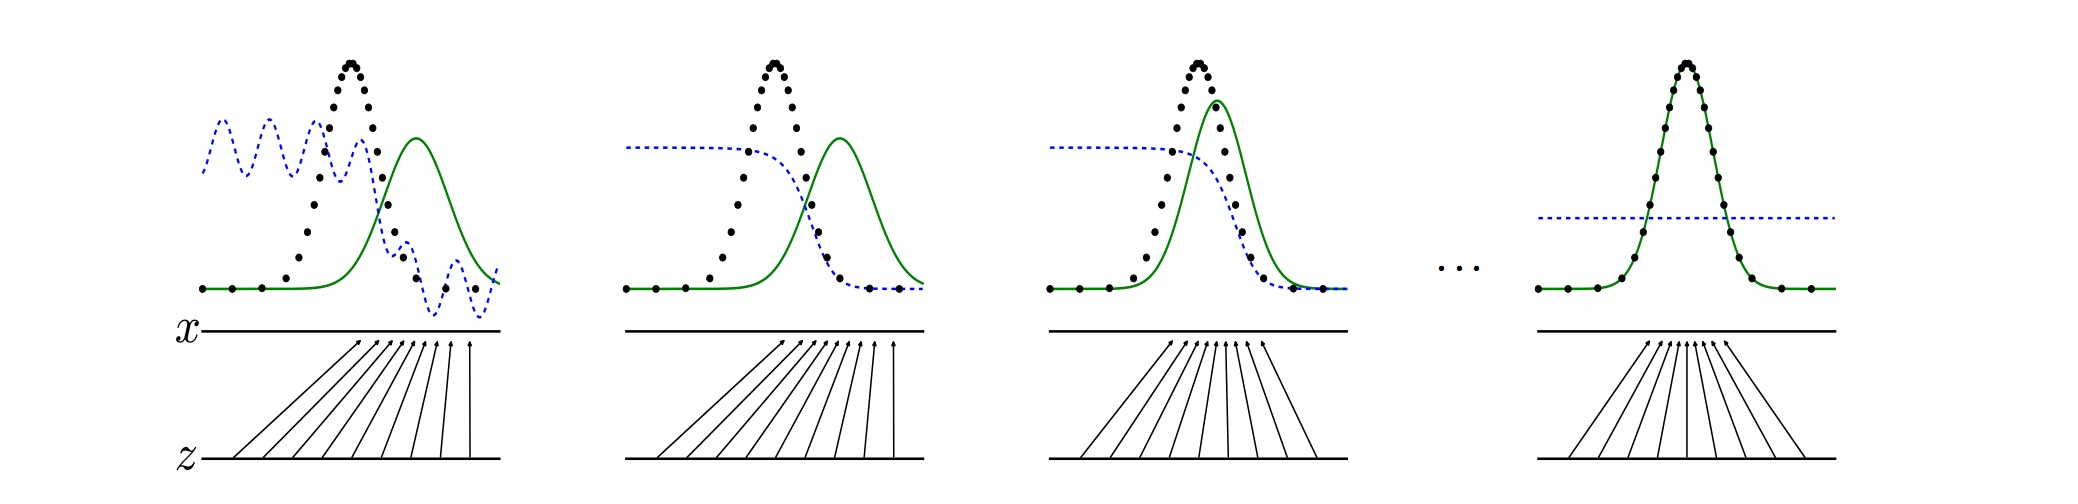
\includegraphics[width=1\textwidth]{adversarial_overview}
    \caption{Generative Adversarial Networks over time, Figure from \cite{goodfellow14}}
    \end{figure}
\end{frame}

\begin{frame}{Generative Adversarial Networks}
    \begin{figure}[h]
    \centering
    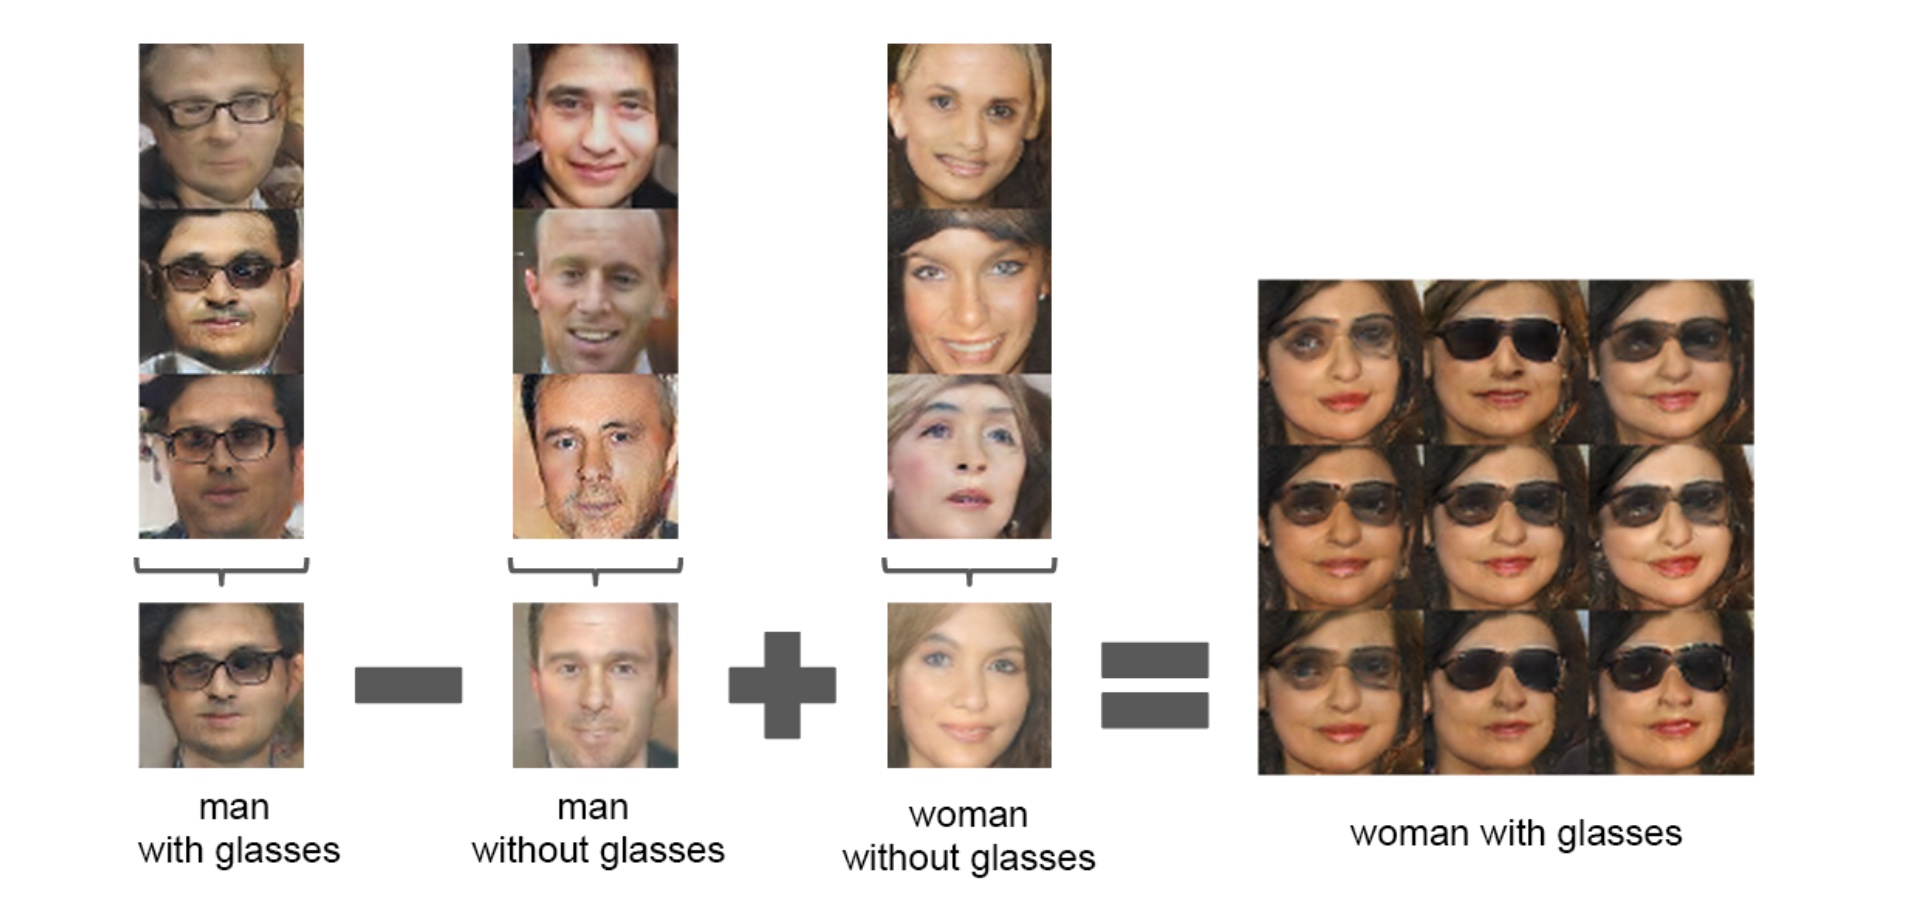
\includegraphics[width=1\textwidth]{vector_arithmetic}
    \caption{vector arithmetic on the generators input, Figure from \cite{Radford15}}
    %Trick: average noise over similiar representations
    \end{figure}
\end{frame}

\begin{frame}{Generative Adversarial Networks}
    \begin{figure}[h]
    \centering
    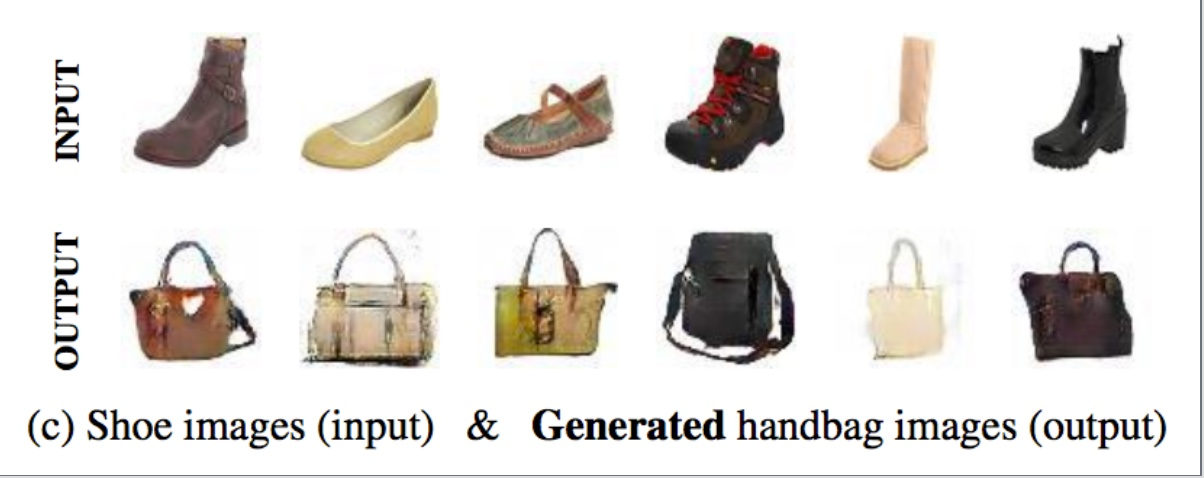
\includegraphics[width=1\textwidth]{shoe2handbag}
    \caption{Learning cross domain relations between shoes and handbags, Figure from \cite{Kim17}}
    \end{figure}
\end{frame}

\section{Comparison}
\subsection{Comparison}
\begin{frame}{Comparison to usual neural networks}
    \textbf{the traditional approach:}\\
    While other approaches exist (for example variational autoencoders \cite{KingmaW13}), 
    most of the applications of neural networks are of an discriminative nature, for example classification.
    Generative models open up exciting new possibilites.
\end{frame}

\section{Convolutional Neural Networks}
\begin{frame}
    \vfill
    \centering
    \begin{beamercolorbox}[sep=8pt,center,shadow=true,rounded=true]{title}
      \usebeamerfont{title}Convolutional Neural Networks
    \end{beamercolorbox}
    \vfill
\end{frame}

\begin{frame}{Convolutional Neural Networks}
    \begin{figure}[h]
        \centering
        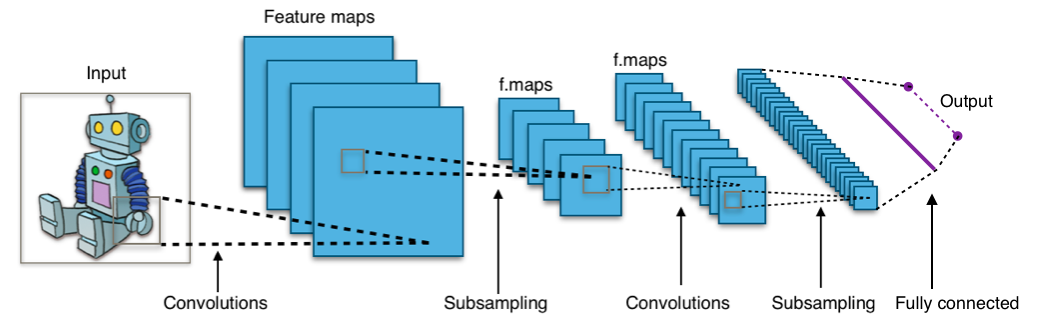
\includegraphics[width=1\textwidth]{Typical_cnn.png}
        \end{figure}
\end{frame}

\begin{frame}{Convolutional Neural Networks}
    \begin{figure}[h]
        \centering
        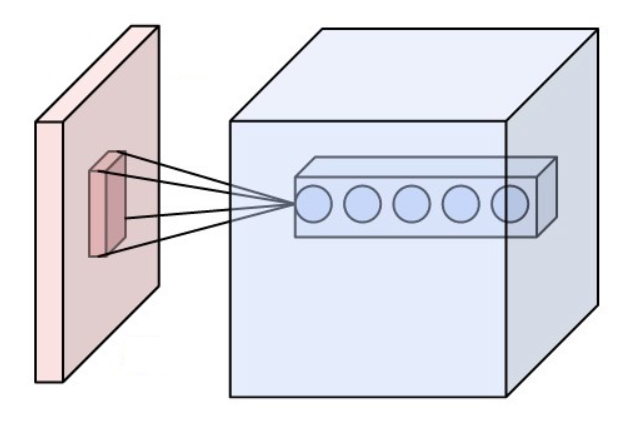
\includegraphics[width=1\textwidth]{Conv_layer.png}
        \end{figure}
\end{frame}

\begin{frame}{Convolutional Neural Networks}
    \begin{figure}[h]
        \centering
        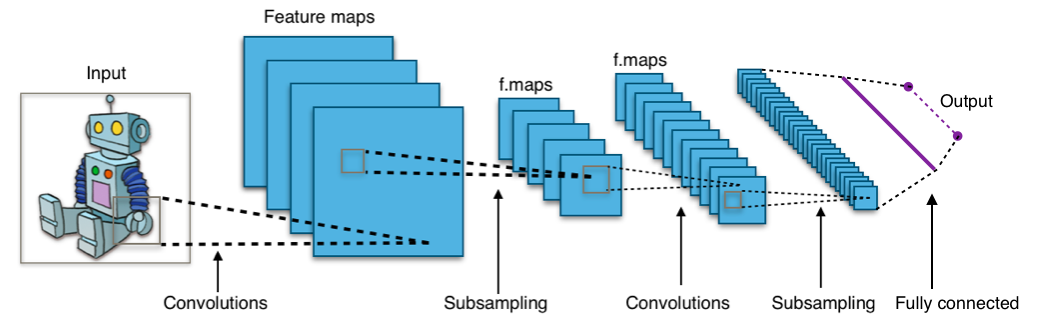
\includegraphics[width=1\textwidth]{Typical_cnn.png}
        \end{figure}
\end{frame}

\appendix
\beginbackup

\begin{frame}[allowframebreaks]{References}
%\begin{thebibliography}{9}
    %\bibitem{Mirza14}
    %Mehdi Mirza, Simon Osindero,
    %\emph{Conditional Generative Adversarial Nets},
    %arXiv preprint 	arXiv:1411.1784,
    %2014.

%\end{thebibliography}
\printbibliography
\end{frame}

\backupend

\end{document}
